\subsection{Single-Line Diagrams (SLD)}

\begin{define}
    \textbf{Single-line diagram:} representation of an electrical system, providing a view of its components, interconnections, and electrical flow paths

    \textbf{Bus:} in an electrical system, this is a node where several line or several lines are connected. In power systems specifically, this is any garph node of the single-line diagram at which voltage, curernt, power flow or other quantities can be evaluated
\end{define}
\textbf{More detailed explanation from Schematic Representation of Power System Relaying report:}

Shows the overall scheme and connections and interactions between equipment and relay system components but in a simplified manner. For example, it uses a single line to represent three phases (hence the name “single line”). The information is shown schematically, but the high- voltage portion is usually shown in a pseudo-physical layout that matches or mimics the actual bus layout in the substation. All relays and other major components are assigned a unique identification. The identification is carried through the entire drawing set. There may be other drawings in the single line format. There may also be a one line diagram that emphasizes the power system equipment and does not detail the relay system components but only those elements connected directly at the primary voltage. This may be referred to as the “station”, “station one line”, or “power one line” diagram. There may also be a simplified one line diagram showing all the protection schemes and their intended zones of protection. This is referred to as the “protection zone” or “meter and relay single line” diagram.

\textbf{Components on a single-line diagram}
\begin{itemize}
    \item Power sources - includes generators, utility supplies and indicates their voltage levels and connection points to the electrical system
    \item Electrical Equipment - includes transformers, circuit breakers, switches, motors, and loads
    \item Bus arrangement - includes bus bars for power distribution at different voltage levels and shows how power is routed from one location to another
    \item Protective devices - includes fuses, circuit breakers, and relays
    \item Metering/instrumentation - includes metering devices (ammeter, voltmeter etc) and measuring points for monitoring/control
\end{itemize}

Bus Arrangement and Voltage Levels
\begin{define}
    Bus duct  
    \begin{itemize}
        \item Carries high currents between different electrical components and sections
        \item Ensures efficient power distribution and reduce
    \end{itemize}
    Transformer 
    \begin{itemize}
        \item Used to step down or setp up voltage levels
        \item Placed at locations to convert high-voltage power from the utility grid to lower voltages or to increase voltage for long-distance Transmission
        \item Winding figurations, type, kVA ratings, cool methods, and surge/lightning protection devices are listed
    \end{itemize}
    Voltage/current transformers (VT, CT)
    \begin{itemize}
        \item Used to measure voltage and current levels for metering, protection, and control purposes
    \end{itemize}
\end{define}

Single line diagrams are the most simplified schematic and least detailed since they rely on basic symbols. We can list a drawing hierarchy from least to most detailed.
\begin{enumerate}
    \item Single line
    \item AC/DC schematics
    \item Logic/wiring diagrams
\end{enumerate}
Each type of schematic has different meaning depending on the intended use. Day to day activities associated with power system work include planning, designing, managing, estimating, commissioning, testing, operating, maintaining, consulting, and providing legal records. The activities are performed by personnel from different organizational groups such as attorneys, project managers, electricians, relay technicians, design engineers, substation operators, system dispatchers, and system planners. How each function is situated within the organizational structure of a power system operator might impact how the different types of drawings are combined and used. Certain functions such as real time power system operation have very high priority when compared to activities such as accounting that can be done at any time after the fact. This is then reflected into the level of detail contained by each type of drawing depending upon its purposes and priorities.

\subsubsection{Symbols}
It is difficult to keep a SLD easy to read while including all the necessary data. We want to communicate function using symbols
\begin{figure}[H]
    \centering
    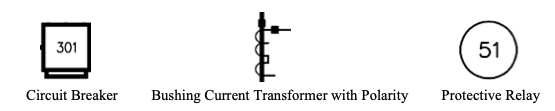
\includegraphics[scale = 0.5]{figs/sld_symbol.png}
    \caption{Examples of symbols used on one line diagrams}
    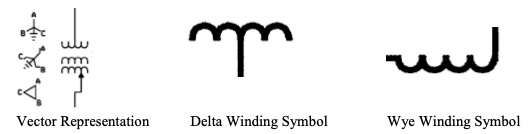
\includegraphics[scale = 0.5]{figs/sld_3phase.png}
    \caption{Three phase connection in a SLD}
\end{figure}

More symbols loaded below

\includepdf[pages={5,6,7,8,9,10}]{daltco_wiring_guide}